\section{Lesson Transcript}
%-- Message Achilleas ( moderator )
% Hi, everyone!

%------------------
%-- Message MTHJJS ( user )
% Hi!

%------------------
%-- Message MeepMurp5 ( user )
% Hi

%------------------
%-- Message bryanguo ( user )
% Hi!

%------------------
%-- Message pritiks ( user )
% hello!

%------------------
%-- Message mark888 ( user )
% Hi!

%------------------
%-- Message leoouyang ( user )
% hello

%------------------
%-- Message ca981 ( user )
% Hi!

%------------------
%-- Message Achilleas ( moderator )
% \textbf{Olympiad GeometryWeek 12: Inversion}

%------------------
%-- Message Achilleas ( moderator )
% As this is the last class, don't forget to fill out your feedback form on the class homepage! Your ideas and suggestions help us make AoPS even more amazing than it already is.

%------------------
%-- Message Achilleas ( moderator )
In our first 11 classes we discussed tactics and approaches which, while not always completely straightforward, can be demystified by a little experience.  Many of them were intuitively clear (though the problems we worked might still be quite challenging).

%------------------
%-- Message Achilleas ( moderator )
Above all, there wasn't anything magical about our tools - we could see them and understand them pretty well, and it didn't require any great leaps of faith or genius to use them.

%------------------
%-- Message Achilleas ( moderator )
For example, the geometric transformations we've discussed - dilation (homothety), reflection, rotation - we have a physical feel for.

%------------------
%-- Message Achilleas ( moderator )
Today, we take a step outside that nice safe realm and into an area that might feel a little like magic at first.

%------------------
%-- Message Achilleas ( moderator )
Today, we talk about the \textbf{geometric transformation inversion}.

%------------------
%-- Message Achilleas ( moderator )
Inversion, as you'll see, is fairly limited in the problems it can be applied to, but when it's useful it usually blows apart a problem pretty quickly.

%------------------
%-- Message Achilleas ( moderator )
The statement of inversion is pretty simple.  In reflection, we reflect over a line.  In inversion, we `reflect' over a circle.

%------------------
%-- Message Achilleas ( moderator )
\begin{definition}
Specifically, if we have a circle with center $O$ and radius $r$, the image of point $P$ upon inversion about the circle is the point $P'$ on ray $OP$ such that $OP\cdot OP' = r^2$.    
\end{definition}

%------------------
%-- Message Achilleas ( moderator )



\begin{center}
\begin{asy}
import cse5;
import olympiad;
// unitsize(4cm);

size(250);
pen s = fontsize(8);

/* helper functions */
path scale(real s, pair D, pair E, real p) { return (point(D--E,p)+scale(s)*(-point(D--E,p)+D)--point(D--E,p)+scale(s)*(-point(D--E,p)+E));}
pair r(pair A, pair B, real d){return B+rotate(d)*(A-B);}

real t = .4;
pair O = origin, X = dir(0), P = point(O--X,t), PP = scale(1/(t))*X;
draw(Circle(O,1),heavygreen);
draw(O--scale(1.1)*PP);
dot(MP("O",O,S,s)^^MP("P",P,S,s)^^MP("X",X,SE,s)^^MP("P'",PP,S,s));
draw(brace(shift((0,.05))*O, shift((0,.05))*X)^^MP("r",point(O--X,.5),6N,s));

\end{asy}
\end{center}





%------------------
%-- Message Achilleas ( moderator )
What is the inverse of P' with respect to the circle?

%------------------
%-- Message RP3.1415 ( user )
% $P$

%------------------
%-- Message Ezraft ( user )
% $P$

%------------------
%-- Message Gamingfreddy ( user )
% P

%------------------
%-- Message Yufanwang ( user )
% P

%------------------
%-- Message ca981 ( user )
% P

%------------------
%-- Message mark888 ( user )
% P

%------------------
%-- Message coolbluealan ( user )
% P

%------------------
%-- Message sae123 ( user )
% P

%------------------
%-- Message mustwin_az ( user )
% P

%------------------
%-- Message bryanguo ( user )
% P

%------------------
%-- Message Trollface60 ( user )
% P

%------------------
%-- Message J4wbr34k3r ( user )
% P

%------------------
%-- Message MeepMurp5 ( user )
% P

%------------------
%-- Message MathJams ( user )
% P

%------------------
%-- Message Achilleas ( moderator )
We know that point $P$ is on ray $OP'$ and that $OP \cdot OP' = r^2$, so $P$ is the inverse of $P'$.  Hence, like reflection and 180-degree rotations, the transformation inversion has a period of 2 (which means that if we apply it twice, everything is back where it started in the end).

%------------------
%-- Message Achilleas ( moderator )
\vspace{6pt}
When we work with a transformation (like homothety, reflection, rotation, and now inversion), what are some easy questions we can ask that will help us understand our transformation?

%------------------
%-- Message sae123 ( user )
% are angles or lengths preserved?

%------------------
%-- Message dxs2016 ( user )
% are lengths/angles preserved

%------------------
%-- Message pritiks ( user )
% where does the transformation map the points/lines?

%------------------
%-- Message MTHJJS ( user )
% 1. keep distance or not?  2. What happens with whole shapes?

%------------------
%-- Message JacobGallager1 ( user )
% What angles does it preserve?

%------------------
%-- Message Yufanwang ( user )
% Is a shape always mapped to a similar shape?

%------------------
%-- Message MathJams ( user )
% where does circles/lines go under inversion?

%------------------
%-- Message Ezraft ( user )
% Is there an identity (a point which the inversion maps to itself)

%------------------
%-- Message Achilleas ( moderator )
1. We can figure out what points are fixed under the transformation. 


2. We can figure out what figures (lines, circles, etc) are fixed.


3. We can think about how to construct the image of a point.


4. We can think about what happens when we transform figures like circles and lines.


5. We can think about what quantities remain constant under the transformation.

%------------------
%-- Message Achilleas ( moderator )
\begin{remark}
Notice that most of these involve figuring what remains the same under the transformation - this is where much of the usefulness of any sort of transformation (even transformations outside geometry, such as algebraic transformations) comes from.  Understanding what remains fixed is often the key to understanding the transformation.    
\end{remark}

%------------------
%-- Message Achilleas ( moderator )
So, we'll start with points.  What points are fixed?  (In other words, for what points P is the inverse of P also P?)

%------------------
%-- Message MeepMurp5 ( user )
% points on the circle

%------------------
%-- Message coolbluealan ( user )
% points on the circle

%------------------
%-- Message J4wbr34k3r ( user )
% Any point on the original circle.

%------------------
%-- Message Gamingfreddy ( user )
% All points on the circle

%------------------
%-- Message JacobGallager1 ( user )
% Points on the circle

%------------------
%-- Message mark888 ( user )
% points on the circle

%------------------
%-- Message SlurpBurp ( user )
% points on the circle

%------------------
%-- Message Wangminqi1 ( user )
% When $P$ is on the circle

%------------------
%-- Message Riya_Tapas ( user )
% When $P$ lies on the circle

%------------------
%-- Message Ezraft ( user )
% all points on the circle

%------------------
%-- Message pike65_er ( user )
% If P lies on the circle

%------------------
%-- Message mustwin_az ( user )
% If P is on circle O

%------------------
%-- Message Achilleas ( moderator )
Only points on the circle map to themselves.  The inverse of a point inside the circle is outside the circle and vice versa (we can see this from $OP \cdot OP' = r^2$: if $OP < r$, then $OP'$ must be greater than $r$ and vice versa).

%------------------
%-- Message Achilleas ( moderator )
What point should we be curious about at this point?

%------------------
%-- Message vsar0406 ( user )
% Point O

%------------------
%-- Message SlurpBurp ( user )
% the center of the circle

%------------------
%-- Message pike65_er ( user )
% the center of the circle

%------------------
%-- Message JacobGallager1 ( user )
% The center of the circle

%------------------
%-- Message MathJams ( user )
% Where does O go?

%------------------
%-- Message sae123 ( user )
% oh where does the center get mapped?

%------------------
%-- Message Achilleas ( moderator )
The center of the circle - what is its inverse?

%------------------
%-- Message MathJams ( user )
% O goes to $P_{\infty}$

%------------------
%-- Message J4wbr34k3r ( user )
% The point at infinity.

%------------------
%-- Message Achilleas ( moderator )
Since OP = 0 when P is the center of the circle, there is no point P' such that $OP \cdot OP' = r^2$.  To get around this, we say that the inverse of the center of the circle is ``the point at infinity", since as P gets closer and closer to O, its inverse gets farther and farther away.  Conversely, the inverse of the ``point at infinity" is the center of our circle.

%------------------
%-- Message Achilleas ( moderator )
You may have heard before that we can add a ``line at infinity" to the Euclidean plane, to obtain the so called real projective plane. That is not what we are doing here. We now add a single ``point at infinity" to the plane. To do this, identify the Euclidean plane to the complex numbers, then add the ``point at infinity" to obtain the so called inversive plane. The inversive plane is also called the complex projective line.

%------------------
%-- Message Achilleas ( moderator )
One way to visualize this is to identify the inversive plane to the Riemann sphere. Imagine that you bend the plane to form a sphere, such that all ends meet at the North Pole of the sphere, which we denote $\infty$. The lines from our plane bend to become circles on the sphere, passing through $\infty$.

%------------------
%-- Message Achilleas ( moderator )
There is a one-to-one map $P$ between the Riemann sphere and the inversive plane, called the stereographic projection. $P(A)$ is just the intersection of the line through $\infty$ and $A$ with our plane. We have $P(\infty)=\infty$. Note that the circles through $\infty$ become lines in the plane.

%------------------
%-- Message Achilleas ( moderator )
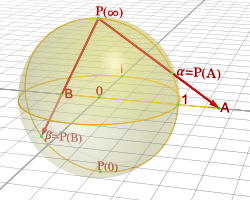
\includegraphics[]{778a917377fe8c15e4e748da260bc93f2bc63e73}
% //cdn.artofproblemsolving.com/images/7/7/8/778a917377fe8c15e4e748da260bc93f2bc63e73.png ]]]

%------------------
%-- Message Achilleas ( moderator )
This means that we can think of lines in the plane as infinite circles (circles through $\infty$ on the Riemann sphere). More on this later.

%------------------
%-- Message Achilleas ( moderator )
What figures are fixed (i.e. what lines/circles/etc map to themselves, even if points on that figure do not map to themselves)?

%------------------
%-- Message bryanguo ( user )
% the circle we perform inversion on is fixed

%------------------
%-- Message Achilleas ( moderator )
Clearly the circle we are inverting about maps to itself, as every point on it maps to itself.

%------------------
%-- Message Achilleas ( moderator )
Are there any other fixed figures?

%------------------
%-- Message Gamingfreddy ( user )
% Lines through the center of the circle

%------------------
%-- Message MathJams ( user )
% Any line through O is fixed

%------------------
%-- Message sae123 ( user )
% any line through the center of the circle maps to itself

%------------------
%-- Message JacobGallager1 ( user )
% Lines through $O$?

%------------------
%-- Message RP3.1415 ( user )
% a line through the center of the circle

%------------------
%-- Message Achilleas ( moderator )
Lines through O (the center of inversion) are fixed.  Make sure you see this.

%------------------
%-- Message Achilleas ( moderator )
There is one more set of non-obvious (but very important) fixed figures.  We'll come back to it soon.

%------------------
%-- Message Achilleas ( moderator )
Next we'll talk about construction.  Thinking about how to construct the diagram for a given problem can help us figure out how to solve the problem (I've solved a surprising number of problems this way).  Similarly, thinking about how to construct the image of a transformation can help us understand the transformation.

%------------------
%-- Message Achilleas ( moderator )
Suppose point P is inside circle with center O.  How do we construct the inverse of P about O?  (Call the inverse P' as usual.)

%------------------
%-- Message Achilleas ( moderator )
What information do we have?

%------------------
%-- Message MathJams ( user )
% $OP\cdot OP' = r^2$

%------------------
%-- Message AOPS81619 ( user )
% $OP\cdot OP'=r^2$

%------------------
%-- Message Trollface60 ( user )
% OP * OP' = r^2

%------------------
%-- Message Achilleas ( moderator )
What else?

%------------------
%-- Message JacobGallager1 ( user )
% $P'$ is on the line $OP$

%------------------
%-- Message pike65_er ( user )
% we know P' lies on line OP

%------------------
%-- Message MeepMurp5 ( user )
% $O, P, P'$ are collinear

%------------------
%-- Message sae123 ( user )
% $O,P,P'$ are collinear

%------------------
%-- Message mustwin_az ( user )
% O,P,P' collinear

%------------------
%-- Message vsar0406 ( user )
% O, P, and P' are collinear

%------------------
%-- Message Catherineyaya ( user )
% $P'$ lies on ray $OP$

%------------------
%-- Message RP3.1415 ( user )
% O, P, P' are collinear

%------------------
%-- Message Achilleas ( moderator )
We know that point P' lives on ray OP, and that $OP \cdot OP' = OX^2$:

%------------------
%-- Message Achilleas ( moderator )
% https://s3.amazonaws.com/classroom.artofproblemsolving.com/Classes/GeomOlympiad/Images/inversion.gif
\begin{center}
    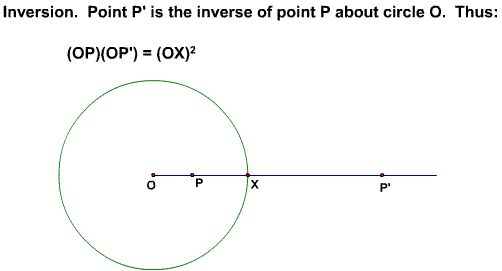
\includegraphics[scale=0.8]{inversion}    
\end{center}
%------------------
%-- Message Achilleas ( moderator )
So we can start our construction by drawing ray OP.  Now we have to find P'.  What tools are we likely to use?

%------------------
%-- Message leoouyang ( user )
% Power of Point

%------------------
%-- Message sae123 ( user )
% Kind of reminds me of power of a point

%------------------
%-- Message SlurpBurp ( user )
% similar triangles?

%------------------
%-- Message MTHJJS ( user )
% similarity

%------------------
%-- Message Ezraft ( user )
% power of a point

%------------------
%-- Message xyab ( user )
% power of a point?

%------------------
%-- Message MathJams ( user )
% Power of a point

%------------------
%-- Message Achilleas ( moderator )
We seek the point P' such that $OP \cdot OP' = OX^2$.  The obvious candidates are power of a point and similar triangles.

%------------------
%-- Message Achilleas ( moderator )
If we try power of a point, we'll want to draw a circle passing through P and P', and we'll want the tangent from O to hit that circle somewhere on the green circle.  But given only P (not P' ), it's not clear how we construct this circle.

%------------------
%-- Message Achilleas ( moderator )
So we turn to similar triangles.  But what's the problem with that?

%------------------
%-- Message Trollyjones ( user )
% there are no triangles to work with

%------------------
%-- Message Trollface60 ( user )
% no triangles

%------------------
%-- Message Gamingfreddy ( user )
% We don't have triangles

%------------------
%-- Message sae123 ( user )
% no triangles!

%------------------
%-- Message MathJams ( user )
% We don't have any triangles!

%------------------
%-- Message MeepMurp5 ( user )
% there aren't any, so we need to make them

%------------------
%-- Message mustwin_az ( user )
% No triangles or angles

%------------------
%-- Message smileapple ( user )
% we don't have any triangles

%------------------
%-- Message Catherineyaya ( user )
% there are no triangles

%------------------
%-- Message xyab ( user )
% we dont have triangles

%------------------
%-- Message Achilleas ( moderator )
No triangles.

%------------------
%-- Message Achilleas ( moderator )
Hmm. . .  So we think maybe we should build triangles.  What kind of triangles should we think of building?

%------------------
%-- Message Gamingfreddy ( user )
% Right triangles

%------------------
%-- Message MeepMurp5 ( user )
% probably right triangles

%------------------
%-- Message dxs2016 ( user )
% right triangles?

%------------------
%-- Message xyab ( user )
% right triangles

%------------------
%-- Message ca981 ( user )
% right triangle

%------------------
%-- Message Trollyjones ( user )
% right triangles

%------------------
%-- Message Achilleas ( moderator )
We think to try building right triangles since they often give us similar triangles.  Right triangles.  Circle.  Point outside the circle.  Does anyone want to take a guess at how to construct P' now?

%------------------
%-- Message J4wbr34k3r ( user )
% The tangents from P' to the circle intersect it at the points the line passing through P and perpendicular to OP intersect the circle.

%------------------
%-- Message Achilleas ( moderator )
We think `Right triangles.  Circle.  Point outside the circle.  Let's draw tangents.  We need to incorporate P somehow, so maybe P is the intersection of OP' and the segment connecting the points of tangency when we draw the tangents through P'

%------------------
%-- Message MathJams ( user )
% Construct a line perpendicular to $OX$ through $P$ and let it intersect the circle at $A$ and $B$, and construct $P'$ by extending a line tangent to the circle at A and finding it's intersection with ray $OX$

%------------------
%-- Message Achilleas ( moderator )
Are we right?  Is P' the intersection of ray OP and the tangent to the circle at point A as shown in the diagram?

%------------------
%-- Message Achilleas ( moderator )



\begin{center}
\begin{asy}
import cse5;
import olympiad;
// unitsize(4cm);

size(250);
pen s = fontsize(8);

/* helper functions */
path scale(real s, pair D, pair E, real p) { return (point(D--E,p)+scale(s)*(-point(D--E,p)+D)--point(D--E,p)+scale(s)*(-point(D--E,p)+E));}
pair r(pair A, pair B, real d){return B+rotate(d)*(A-B);}

real t = .4;
pair O = origin, X = dir(0), P = point(O--X,t), PP = scale(1/(t))*X;
pair A = tangent(PP,O,1,1), B = tangent(PP,O,1,2);

draw(Circle(O,1),heavygreen);
draw(O--scale(1.1)*PP);
dot(MP("O",O,S,s)^^MP("P",P,SE,s)^^MP("X",X,SE,s)^^MP("P'",PP,S,s));
draw(O--MP("A",A,N,s)--PP--MP("B",B,S,s)--cycle^^A--B);
draw(rightanglemark(O,A,PP,3)^^rightanglemark(O,P,A,3)^^rightanglemark(O,B,PP,3),heavyred);

\end{asy}
\end{center}





%------------------
%-- Message pritiks ( user )
% yes

%------------------
%-- Message Achilleas ( moderator )
Why?

%------------------
%-- Message Achilleas ( moderator )
How do we know that $OP\cdot OP'=OX^2$ in the above figure?

%------------------
%-- Message smileapple ( user )
% similar triangles $\triangle OPA\sim\triangle OAP'$

%------------------
%-- Message Lucky0123 ( user )
% Because due to similar triangles $\triangle POB$ and $\triangle PBP',$ we know that $OP * OP' = OX^2$

%------------------
%-- Message MathJams ( user )
% Because $\triangle OAP\sim \triangle OP'A \implies \frac{OA}{OP}=\frac{OP'}{OA}\implies OA^2=OP\cdot OP'=OX^2$

%------------------
%-- Message Catherineyaya ( user )
% $\triangle APO\sim\triangle P'AO$ so $OP/AO=AO/OP'$ and $OP\cdot OP'=OA^2=OX^2$

%------------------
%-- Message ca981 ( user )
% triangle AOP and P'OA are similar

%------------------
%-- Message coolbluealan ( user )
% $\triangle OPA \sim \triangle OAP'$

%------------------
%-- Message JacobGallager1 ( user )
% $\triangle OPA \sim \triangle APP' \sim \triangle OAP'$, so $\frac{OP}{OX} = \frac{OX}{OP'}$

%------------------
%-- Message Gamingfreddy ( user )
% Triangles OAP and OP'A are similar, so OP/AO = AO/OP' -> OP * OP' = (OX)^2 since AO = OX

%------------------
%-- Message Ezraft ( user )
% because $\triangle OPA \sim \triangle OAP',$ $\frac{OP}{OA} = \frac{OA}{OP'}$ and since $OA = OX,$ we see that $OP \cdot OP' = OX^2$

%------------------
%-- Message Achilleas ( moderator )
Since $\triangle OAP \sim \triangle OP'A$, we have $\dfrac{OP'}{OA} = \dfrac{OA}{OP}$, or $OP \cdot OP' = OA^2$.  $OA$ is a radius, so we have our desired relationship.  $P'$ is the intersection of ray $OP$ and the tangent to the circle at point $A$ as shown in the diagram.  How do we do our construction starting from the original $P$?

%------------------
%-- Message MathJams ( user )
% We can construct a line perpendicular to $OX$ through $P$ and let it intersect the circle at $A$ and $B$, and construct $P'$ by extending a line tangent to the circle at A and finding it's intersection with ray $OX$

%------------------
%-- Message Achilleas ( moderator )
We simply draw a line perpendicular to OP through P to get A.  Then draw OA, and a line through A perpendicular to OA.  Where this line meets ray OP is our P'.

%------------------
%-- Message Achilleas ( moderator )
Once again, we're seeing that similar triangles are at the heart of one of our powerful geometric tools.

%------------------
%-- Message Achilleas ( moderator )
Next let's talk about what happens when we invert lines and circles.  We already know what happens if we invert the circle we are inverting about - we get that circle back.  We also know that if we invert a line through the center we get that line back.

%------------------
%-- Message Achilleas ( moderator )
What happens if we invert a circle with center O but a different radius?  (Say this circle has radius s and our original circle that we are inverting about has radius r, as usual.)

%------------------
%-- Message coolbluealan ( user )
% we get a circle with center O and radius r^2/s

%------------------
%-- Message J4wbr34k3r ( user )
% A circle with center O and radius $\frac{r^{2}}{s}$

%------------------
%-- Message Gamingfreddy ( user )
% We get a circle with center O and radius r^2/s

%------------------
%-- Message MeepMurp5 ( user )
% circle centered at $O$ with radius $r^2/s$

%------------------
%-- Message dxs2016 ( user )
% OP*OP' = s^2 --> OP' = s^2/OP. if P is point on circumference of circle, length of OP' is fixed --> circle

%------------------
%-- Message pike65_er ( user )
% a circle with radius $\frac{r^2}{s}$ centered at O

%------------------
%-- Message ca981 ( user )
% Another concentric circle with radius = r^2/s

%------------------
%-- Message Achilleas ( moderator )
Every point on the inverse of the circle with radius s will be a distance of $r^2/s$ away from O, since $OP \cdot OP' = r^2$ and $OP = s$ for all points $P$ on the circle with radius $s$.

%------------------
%-- Message Achilleas ( moderator )
Conversely, every point on our inverse circle can be produced by inverting our original circle.

%------------------
%-- Message Achilleas ( moderator )
Hence, our inverse is a circle with radius $r^2/s$.

%------------------
%-- Message Achilleas ( moderator )
Let's try lines that don't pass through the center.  We'll start with one that doesn't even touch the circle:

%------------------
%-- Message Achilleas ( moderator )



\begin{center}
\begin{asy}
import cse5;
import olympiad;
// unitsize(4cm);

pair O, SS, SSP;
O = (0,0);
SS = (1.7,0);
SSP = (1/1.7,0);
unitsize(0.5inch);
defaultpen(black+0.75);
draw(Circle((0,0),1));
draw((1.7,-1.2)--(1.7,2));

\end{asy}
\end{center}





%------------------
%-- Message Achilleas ( moderator )
Any observations?

%------------------
%-- Message J4wbr34k3r ( user )
% A circle passing through O but always inside the original circle.

%------------------
%-- Message MathJams ( user )
% all the points on the line invert to points inside the circle

%------------------
%-- Message JacobGallager1 ( user )
% The image of the line must lie entirely within the circle

%------------------
%-- Message SlurpBurp ( user )
% the image must pass through the center of the circle, because the line contains the point at infinity

%------------------
%-- Message bryanguo ( user )
% if we invert points on that line wrt the circle the points that have been inverted will be inside the circle

%------------------
%-- Message Achilleas ( moderator )
If we invert this line, we know that points arbitrarily close to the center will be in the image, as the line goes infinitely far away from the circle (so the images of those very, very far away points will be very, very close to the center).

%------------------
%-- Message Achilleas ( moderator )
What point on the line will have an image that is farthest from the center of inversion?

%------------------
%-- Message J4wbr34k3r ( user )
% The image of the center when projected onto the line.

%------------------
%-- Message smileapple ( user )
% the projection of the center onto the line

%------------------
%-- Message coolbluealan ( user )
% The point closest to the circle

%------------------
%-- Message dxs2016 ( user )
% the point H where OH is perpendicular to the line

%------------------
%-- Message bryanguo ( user )
% the point on the line which is the foot from the center of the circle to the line

%------------------
%-- Message AOPS81619 ( user )
% The closest point to the circle

%------------------
%-- Message Ezraft ( user )
% the point closest to the circle

%------------------
%-- Message Catherineyaya ( user )
% the point closest to the center

%------------------
%-- Message Wangminqi1 ( user )
% The point on the perpendicular line from the center of the circle

%------------------
%-- Message MathJams ( user )
% the point closest to the circle, or the foot of the perpendicular from the center to the line

%------------------
%-- Message Achilleas ( moderator )
The point that is the inverse of the point on the line closest to the center will be farthest from the center in the image of the line.  This point is the image of the foot of the perpendicular from the center of the circle to the line:

%------------------
%-- Message Achilleas ( moderator )



\begin{center}
\begin{asy}
import cse5;
import olympiad;
// unitsize(4cm);

pair O, SS, SSP;
O = (0,0);
SS = (1.7,0);
SSP = (1/1.7,0);
unitsize(0.5inch);
defaultpen(black+0.75);
draw(Circle((0,0),1));
draw((1.7,-1.2)--(1.7,2));
draw(O--SS);
dot(O,p=black+3);
dot(SSP,p=black+3);
label("$O$",O,S);
label("$S'$",SSP,S);
label("$S$",SS,E);
draw(rightanglemark((1.7,1),SS,O,s=5));

\end{asy}
\end{center}





%------------------
%-- Message Achilleas ( moderator )
Now what?

%------------------
%-- Message MathJams ( user )
% consider another arbitrary point on the line

%------------------
%-- Message dxs2016 ( user )
% try some more points?

%------------------
%-- Message Achilleas ( moderator )
The images of points above S will be above segment OS' and get gradually closer to O.  Those below S will have images below segment OS' and these images will be gradually closer to O.  What might we guess the image of our line is?

%------------------
%-- Message MathJams ( user )
% a circle

%------------------
%-- Message coolbluealan ( user )
% circle

%------------------
%-- Message AOPS81619 ( user )
% A circle

%------------------
%-- Message bryanguo ( user )
% image of our line is a circle

%------------------
%-- Message dxs2016 ( user )
% circle?

%------------------
%-- Message pike65_er ( user )
% a circle

%------------------
%-- Message Achilleas ( moderator )
Inversion seems all about circles and our image is clearly not a line, so we guess that the image is a circle. Which circle it is? Can we be more specific?

%------------------
%-- Message Wangminqi1 ( user )
% The circle with diameter $OS'$

%------------------
%-- Message Gamingfreddy ( user )
% The circle with diameter OS'

%------------------
%-- Message Catherineyaya ( user )
% circle with diameter OS'

%------------------
%-- Message bryanguo ( user )
% circle with diameter $OS'$

%------------------
%-- Message coolbluealan ( user )
% circle with diameter $OS'$

%------------------
%-- Message JacobGallager1 ( user )
% It could be the circle with diameter $OS'$

%------------------
%-- Message AOPS81619 ( user )
% The circle with diameter $OS'$

%------------------
%-- Message dxs2016 ( user )
% circle with diameter OS'?

%------------------
%-- Message Achilleas ( moderator )
It is the circle with diameter OS':

%------------------
%-- Message Achilleas ( moderator )



\begin{center}
\begin{asy}
import cse5;
import olympiad;
// unitsize(4cm);

pair O, SS, SSP;
O = (0,0);
SS = (1.7,0);
SSP = (1/1.7,0);
unitsize(0.5inch);
defaultpen(black+0.75);
draw(Circle((0,0),1));
draw((1.7,-1.2)--(1.7,2));
draw(O--SS);
dot(O,p=black+3);
dot(SSP,p=black+3);
label("$O$",O,SW);
label("$S'$",SSP+(-0.09,0),SE);
label("$S$",SS,E);
draw(rightanglemark((1.7,1),SS,O,s=5));
draw(Circle((O+SSP)/2,length(SSP/2)));

\end{asy}
\end{center}





%------------------
%-- Message Achilleas ( moderator )
How can we prove that the image is this circle?

%------------------
%-- Message coolbluealan ( user )
% pick any point on the line and show that the point's image is on the circle with diameter $OS'$

%------------------
%-- Message smileapple ( user )
% prove all points on a line map to a point on the circle and vice versa

%------------------
%-- Message Achilleas ( moderator )
We must prove that for any point $P$ on the line, the ray $OP$ meets the small circle at a point $P'$ such that $(OP)(OP' ) = r^2$, where $r$ is the radius of circle $O$ (thus the image of $P$ is on the little circle).  How do we do it?

%------------------
%-- Message Lucky0123 ( user )
% Similar triangles

%------------------
%-- Message AOPS81619 ( user )
% Similar triangles

%------------------
%-- Message Achilleas ( moderator )
Similar triangles again give the answer:

%------------------
%-- Message Achilleas ( moderator )



\begin{center}
\begin{asy}
import cse5;
import olympiad;
// unitsize(4cm);

pair O, SS, SSP,P,PP;
O = (0,0);
SS = (1.7,0);
SSP = (1/1.7,0);
PP = SSP/2 + (rotate(80)*(SSP/2));
P = intersectionpoint((1.7,0)--(1.7,2), O -- 7*PP);
unitsize(0.5inch);
defaultpen(black+0.75);
draw(Circle((0,0),1));
draw((1.7,-1.2)--(1.7,2));
draw(O--SS);
dot(O,p=black+3);
dot(SSP,p=black+3);
label("$O$",O,SW);
label("$S'$",SSP+(-0.09,0),SE);
label("$S$",SS,E);
draw(rightanglemark((1.7,1),SS,O,s=5));
draw(Circle((O+SSP)/2,length(SSP/2)));
draw(P--O);
dot(PP,p=black+3);
draw(PP--SSP);
label("$P'$",PP,N);
label("$P$",P,E);

\end{asy}
\end{center}





%------------------
%-- Message Achilleas ( moderator )
How about $\angle OP'S'$?

%------------------
%-- Message pritiks ( user )
% it equals 90 degrees

%------------------
%-- Message dxs2016 ( user )
% 90 degrees

%------------------
%-- Message JacobGallager1 ( user )
% $\angle OP'S' = 90^\circ$

%------------------
%-- Message Wangminqi1 ( user )
% It equals $90^{\circ}$

%------------------
%-- Message coolbluealan ( user )
% it is $90^\circ$

%------------------
%-- Message Ezraft ( user )
% it is a right angle as $OS'$ is a diameter

%------------------
%-- Message AOPS81619 ( user )
% It's 90 degrees

%------------------
%-- Message xyab ( user )
% $\angle OP'S' = 90^{\circ}$

%------------------
%-- Message Achilleas ( moderator )
Angle $OP'S'$ is inscribed in a semicircle, so it's a right angle.  Hence $\triangle OP'S' \sim \triangle OSP$ and we have $\dfrac{OP'}{OS'} = \dfrac{OS}{OP}$, so $OP' \cdot OP = OS \cdot OS' = r^2$, since $S'$ is defined to be the image of point $S$.

%------------------
%-- Message Achilleas ( moderator )
Note that we can use this to show both that the image of any point on the line is on the circle, and that any point on the circle is the image of some point on the line.  We must show both - this is essentially a locus problem so we have to prove it in both directions (all points in the inverse of the line are on the little circle and all points on the little circle are images of points on the line).

%------------------
%-- Message Achilleas ( moderator )
Similarly, all lines that do not pass through the center become circles on inversion (work out the cases of lines that are tangent to the circle and lines that pass through the circle on your own).

%------------------
%-- Message Achilleas ( moderator )
Will all the images of these lines pass through the center of the original circle?

%------------------
%-- Message dxs2016 ( user )
% yes because of point of infinity

%------------------
%-- Message mustwin_az ( user )
% yes

%------------------
%-- Message JacobGallager1 ( user )
% Yes, because all lines contain the point at infinity

%------------------
%-- Message pike65_er ( user )
% yes

%------------------
%-- Message bryanguo ( user )
% yes

%------------------
%-- Message MTHJJS ( user )
% yes

%------------------
%-- Message Gamingfreddy ( user )
% yes

%------------------
%-- Message ca981 ( user )
% yes.

%------------------
%-- Message SlurpBurp ( user )
% yes

%------------------
%-- Message MathJams ( user )
% Yes because of $P_{\infty}$

%------------------
%-- Message coolbluealan ( user )
% yes because of the point at infinity

%------------------
%-- Message mark888 ( user )
% Yes

%------------------
%-- Message Achilleas ( moderator )
Yes - all lines get infinitely far away from the circle, so all their images will go through the center.

%------------------
%-- Message Achilleas ( moderator )
So, what is the image of circles through the center of the circle we're inverting about?

%------------------
%-- Message coolbluealan ( user )
% lines

%------------------
%-- Message pike65_er ( user )
% lines

%------------------
%-- Message Ezraft ( user )
% lines

%------------------
%-- Message MathJams ( user )
% Lines

%------------------
%-- Message Gamingfreddy ( user )
% lines

%------------------
%-- Message ca981 ( user )
% They are all lines

%------------------
%-- Message Achilleas ( moderator )
Since lines map to circles through the center, circles through the center map to lines.  Work out the details on your own. (I'll put a thread on the message board for this discussion.)

%------------------
%-- Message Achilleas ( moderator )
What's left?

%------------------
%-- Message SlurpBurp ( user )
% circles not passing through $O$

%------------------
%-- Message Ezraft ( user )
% circles that don't pass through the center of the circle we are inverting about

%------------------
%-- Message J4wbr34k3r ( user )
% Circles not passing through the center.

%------------------
%-- Message JacobGallager1 ( user )
% Circles which don't pass through the center, and which do not have center $O$

%------------------
%-- Message MathJams ( user )
% Circles that do not go through the center

%------------------
%-- Message Achilleas ( moderator )
Circles not through the center - what is the image of a circle that does not pass through the center of our inversion circle?

%------------------
%-- Message MathJams ( user )
% Another Circle

%------------------
%-- Message JacobGallager1 ( user )
% Another circle?

%------------------
%-- Message J4wbr34k3r ( user )
% Another circle?

%------------------
%-- Message Achilleas ( moderator )
The image of a circle is a circle.

%------------------
%-- Message Achilleas ( moderator )
What tools will we likely use to prove this?

%------------------
%-- Message JacobGallager1 ( user )
% Similar triangles

%------------------
%-- Message bryanguo ( user )
% similar triangles

%------------------
%-- Message pritiks ( user )
% similar triangles

%------------------
%-- Message J4wbr34k3r ( user )
% Similar triangles?

%------------------
%-- Message Achilleas ( moderator )
We'll probably use pretty much the same tools as we used before: similar triangles.

%------------------
%-- Message Achilleas ( moderator )
In the interest of having time for solving problems using inversion, I'll mostly just outline the proof rather than go through it with all the steps.

%------------------
%-- Message Achilleas ( moderator )
We'll take care of the case in which we are inverting a circle that is entirely outside circle O.

%------------------
%-- Message Achilleas ( moderator )
% https://s3.amazonaws.com/classroom.artofproblemsolving.com/Classes/GeomOlympiad/Images/invertcir2.gif

\begin{center}
    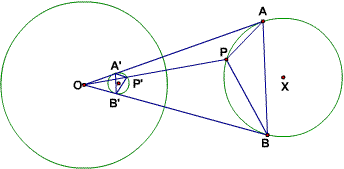
\includegraphics[scale=0.8]{invertcir2}    
\end{center}
%------------------
%-- Message Achilleas ( moderator )
Let circle X be our original circle.  We wish to show that the image of X when inverted about circle O is the little circle shown.  We start with the points of tangency when tangents to circle X from point O are drawn.  These are points A and B.  Let A' and B' be the images of these points.  Hence,

%------------------
%-- Message Achilleas ( moderator )
$$  OA \cdot OA' = OB \cdot OB' = r^2, $$
where r is the radius of circle O.

%------------------
%-- Message Achilleas ( moderator )
We wish to show that the image of point P is on the little circle.

%------------------
%-- Message Achilleas ( moderator )
Let P' be the image of P (so $OP \cdot OP' = r^2$ also).  Given any point P on that arc AB and its image P', what will we have to prove to determine that P' is on that little circle?

%------------------
%-- Message Achilleas ( moderator )
Any ideas?

%------------------
%-- Message MathJams ( user )
% We need to angle chase

%------------------
%-- Message Achilleas ( moderator )
We wish to show that angle $A'P'B'$ is constant (it is $A'B'O$ in particular).  How can we do so?

%------------------
%-- Message Achilleas ( moderator )
We've used similar triangles all over the place today; can we use them here?

%------------------
%-- Message Achilleas ( moderator )
We know that $OA \cdot OA' = OP \cdot OP'$, so $\dfrac{OA}{OP} = \dfrac{OP'}{OA'}$.  Since $\angle A'OP' = \angle POA$, we have $\triangle OAP \sim OP'A'$.  How does this help?  (Remember, we want to prove something about $\angle A'P'B'$.)

%------------------
%-- Message coolbluealan ( user )
% $\angle OP'A'=\angle OAP$

%------------------
%-- Message Achilleas ( moderator )
Focusing on the angle we care about (or part of it), we see that $\angle A'P'O = \angle PAO$ from our triangle similarity.  Hence, $\angle A'P'O = (\text{arc }AP)/2$.

%------------------
%-- Message Achilleas ( moderator )
Now what?

%------------------
%-- Message MathJams ( user )
% $\angle OP'B'=\angle OBP$

%------------------
%-- Message Achilleas ( moderator )
We can do the same for $B'P'O$: $\triangle B'P'O \sim \triangle PBO$, so $\angle B'P'O = \angle PBO = (\text{arc } PB)/2$.  So?

%------------------
%-- Message pritiks ( user )
% angle A'P'B' is constant

%------------------
%-- Message Achilleas ( moderator )
% Why?

%------------------
%-- Message coolbluealan ( user )
% $\angle A'P'B'=(arc AP)/2+(arc BP)/2=(arc AB)/2$

%------------------
%-- Message MathJams ( user )
% Show $\angle A'P'B' = \angle A'OP'+\angle OP'B'=\angle APB$

%------------------
%-- Message dxs2016 ( user )
% angle A'P'B = angle OAP + angle OBP = (arc AB) /2

%------------------
%-- Message Achilleas ( moderator )
$\angle A'P'B' = \angle A'P'O + \angle B'P'O = (\text{arc }AP + \text{arc }PB)/2 = (\text{arc }AB)/2$, which is a constant  Hence, $P'$ is on an arc of a circle through $A'$ and $B'$.

%------------------
%-- Message Achilleas ( moderator )
What else would we have to do to finish the proof?

%------------------
%-- Message Lucky0123 ( user )
% Show that all points on the circle are acquirable

%------------------
%-- Message Achilleas ( moderator )
We'd have to take care of the case in which $P$ is on the major arc $AB$, showing that it leads to a $P'$ such that $A'P'B'$ is the supplement of the $A'P'B'$ found above (thus it is on the same circle, just on the other `side' of $A'B'$ ).  We'd also have to show that every $P'$ is in the image upon inversion of circle $X$.

%------------------
%-- Message Achilleas ( moderator )
The details of that proof are essentially the same as the proof we just did.

%------------------
%-- Message Achilleas ( moderator )
Hence, the inverse of a circle that does not pass through the center of the circle we're inverting about is another circle.

%------------------
%-- Message Achilleas ( moderator )
\bigskip
\centerline{\rule{13cm}{0.4pt}}
Here's a quick summary of what happens to some things we've found.

%------------------
%-- Message Achilleas ( moderator )
1. Lines through the center of inversion go to themselves.

%------------------
%-- Message Achilleas ( moderator )
2. Lines not through the center of inversion go to circles that pass through the center of inversion.

%------------------
%-- Message Achilleas ( moderator )
3. Circles through the center of inversion go to lines (that don't pass through the center of inversion).

%------------------
%-- Message Achilleas ( moderator )
4. Circles not through the center of inversion go to circles not through the center of inversion.

\centerline{\rule{13cm}{0.4pt}}
\bigskip
%------------------
%-- Message Achilleas ( moderator )
In the so-called inversive plane (the plane with our point at infinity added), it's often convenient to think of lines as circles that pass through the point at infinity.

%------------------
%-- Message Achilleas ( moderator )
Using this abuse of notation, all these results can be summarized as follows: inversion takes circles to circles.

%------------------
%-- Message Achilleas ( moderator )
Whether they're bona-fide circles or actually lines that we're pretending are circles depends on whether the ``circle" in question passes through the point at infinity.

%------------------
%-- Message Achilleas ( moderator )
By the way, usually lines intersect at only one point. But circles typically intersect at two points, if they intersect at all.

%------------------
%-- Message Achilleas ( moderator )
So in our inversion scheme where lines are actually circles, shouldn't there typically be two intersection points? What's going on?

%------------------
%-- Message Achilleas ( moderator )
Where is the missing intersection point?

%------------------
%-- Message MeepMurp5 ( user )
% the point at infinity

%------------------
%-- Message JacobGallager1 ( user )
% One of those points is the point at infinity

%------------------
%-- Message SlurpBurp ( user )
% the other point is $P_\infty$?

%------------------
%-- Message Ezraft ( user )
% at infinity

%------------------
%-- Message Achilleas ( moderator )
Right! Every pair of lines is considered to intersect at the point at infinity.

%------------------
%-- Message Achilleas ( moderator )
We even say that parallel lines are tangent at the point at infinity!

%------------------
%-- Message Achilleas ( moderator )
So in inversive geometry land, every pair of lines intersects. (In fact, lines always intersect twice, but maybe twice at the same point---like a polynomial having a repeated root.)

%------------------
%-- Message Achilleas ( moderator )
In a certain sense, it's 1-dimensional complex projective geometry.

%------------------
%-- Message Achilleas ( moderator )
\bigskip
Now we'll talk about what is \textbf{preserved} when we take inversions.

%------------------
%-- Message Achilleas ( moderator )
Is length preserved (i.e. if $A'$ and $B'$ are the inverse of $A$ and $B$, is $A'B' = AB$)?

%------------------
%-- Message MathJams ( user )
% No

%------------------
%-- Message SlurpBurp ( user )
% no

%------------------
%-- Message coolbluealan ( user )
% No

%------------------
%-- Message ca981 ( user )
% NO

%------------------
%-- Message smileapple ( user )
% no?

%------------------
%-- Message JacobGallager1 ( user )
% No

%------------------
%-- Message mustwin_az ( user )
% No

%------------------
%-- Message Trollyjones ( user )
% no

%------------------
%-- Message leoouyang ( user )
% No?

%------------------
%-- Message Gamingfreddy ( user )
% no

%------------------
%-- Message Ezraft ( user )
% no

%------------------
%-- Message Achilleas ( moderator )
No, length is not preserved in general.  Take $A$ to be on the circle and $B$ to be very close to the center - then $A'B'$ can be arbitrarily long.  (Or put $A$ and $B$ both very close to the center such that the center is on segment $AB$ - their images will be very far apart.)

%------------------
%-- Message Achilleas ( moderator )
How about \textbf{angles}?  What do we need to define to talk about angles?

%------------------
%-- Message Ezraft ( user )
% angles made by the intersection of two circles

%------------------
%-- Message Achilleas ( moderator )
First we need a way to talk about angles formed by intersecting circles.  What is a good way to assign an angle measure to how two intersecting circles meet?

%------------------
%-- Message coolbluealan ( user )
% angle formed by the tangents at the intersection point

%------------------
%-- Message Achilleas ( moderator )
We call the angle between the tangents at the intersection point of the circles the angle between the two circles.  (Generally, we'll use the acute angle, assuming the tangents aren't perpendicular.)

%------------------
%-- Message Achilleas ( moderator )
% https://s3.amazonaws.com/classroom.artofproblemsolving.com/Classes/GeomOlympiad/Images/intcir.gif
\begin{center}
    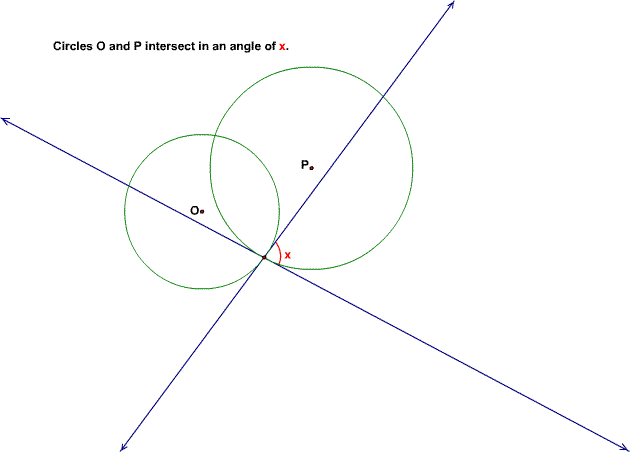
\includegraphics[scale=0.5]{intcir}    
\end{center}
%------------------
%-- Message Achilleas ( moderator )
If the tangents are perpendicular, we call the circles \textbf{orthogonal}.  Circles which are tangent intersect in a 0 degree angle.

%------------------
%-- Message Achilleas ( moderator )
Now that we have a definition for the angle between two circles, we can investigate whether angles are preserved.  Consider first an inversion about a circle centered at the intersection point of the two circles.  What happens?  (I've left in the tangent lines so we can talk about angles.)

%------------------
%-- Message Achilleas ( moderator )
% https://s3.amazonaws.com/classroom.artofproblemsolving.com/Classes/GeomOlympiad/Images/interinv.gif
\begin{center}
    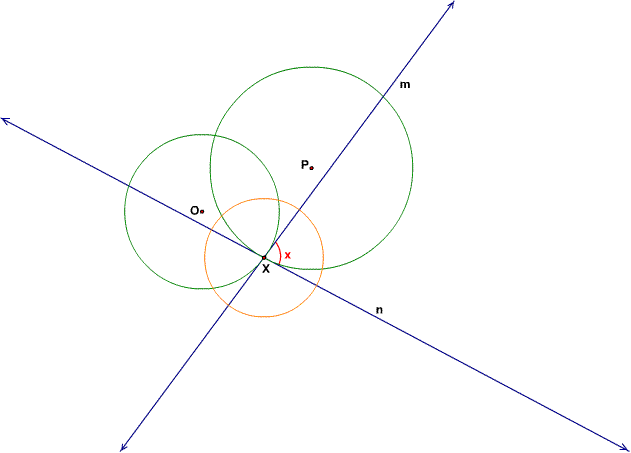
\includegraphics[scale=0.5]{interinv}    
\end{center}
%------------------
%-- Message Achilleas ( moderator )
Suppose we invert about the orange circle X in the diagram, which has a center at X, one of the points of intersection of our green circles.  What is the image of circle P?

%------------------
%-- Message dxs2016 ( user )
% line

%------------------
%-- Message Riya_Tapas ( user )
% a line

%------------------
%-- Message Ezraft ( user )
% a line

%------------------
%-- Message mustwin_az ( user )
% A line

%------------------
%-- Message Achilleas ( moderator )
The image of circle P is a line since P goes through the center of our circle of inversion (point X).  Specifically what line?

%------------------
%-- Message JacobGallager1 ( user )
% It is the radical axis of the orange circle and circle P

%------------------
%-- Message Gamingfreddy ( user )
% the line through the intersections of circle P and the orange circle

%------------------
%-- Message coolbluealan ( user )
% radical axis of circle P and circle X

%------------------
%-- Message Achilleas ( moderator )
The points where circle P and circle X intersect must be in the image, so the line goes through those points.

%------------------
%-- Message Achilleas ( moderator )
Similarly, the image of O is a line through the points of intersection of O and X:

%------------------
%-- Message Achilleas ( moderator )
% https://s3.amazonaws.com/classroom.artofproblemsolving.com/Classes/GeomOlympiad/Images/consangl.gif
\begin{center}
    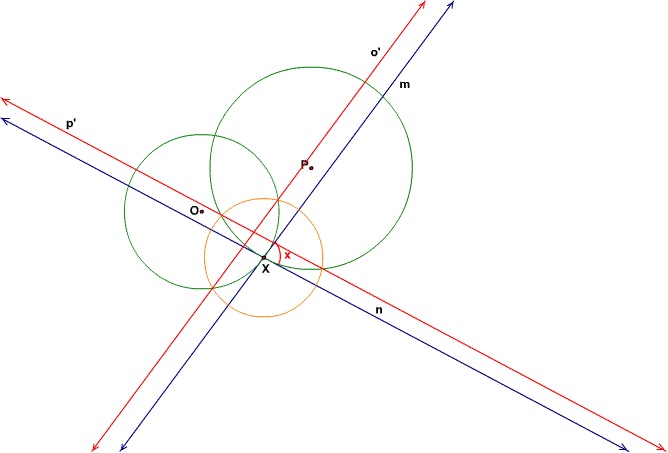
\includegraphics[scale=0.5]{consangl}    
\end{center}
%------------------
%-- Message Achilleas ( moderator )
Line $p'$ is the image of circle $P$ and line $o'$ is the image of circle $O$.  See anything interesting?

%------------------
%-- Message coolbluealan ( user )
% parallel lines

%------------------
%-- Message pritiks ( user )
% the lines are parallel

%------------------
%-- Message Achilleas ( moderator )
% Which lines are parallel?

%------------------
%-- Message Lucky0123 ( user )
% m is parallel to o' and n is parallel to p'

%------------------
%-- Message bryanguo ( user )
% $p' \parallel n$ and $o' \parallel m$

%------------------
%-- Message MathJams ( user )
% o'//m and p'//n

%------------------
%-- Message pritiks ( user )
% p' || n and o'|| m

%------------------
%-- Message Achilleas ( moderator )
It looks like $p' \parallel n$ and $o' \parallel m$.  Is it true?

%------------------
%-- Message Lucky0123 ( user )
% Yes

%------------------
%-- Message mustwin_az ( user )
% yes

%------------------
%-- Message coolbluealan ( user )
% yes

%------------------
%-- Message bryanguo ( user )
% yes

%------------------
%-- Message RP3.1415 ( user )
% yes

%------------------
%-- Message Gamingfreddy ( user )
% Yes

%------------------
%-- Message Achilleas ( moderator )
Since $n$ is tangent to circle $P$, we know that $n$ is perpendicular to $XP$.  We also know that $p'$ is perpendicular to $XP$ since it is a common chord.  Hence $n \parallel p'$.  Similarly, $o' \parallel m$.  So what do we conclude?

%------------------
%-- Message coolbluealan ( user )
% inversion centered on an intersection point between 2 circles preserves angles

%------------------
%-- Message AOPS81619 ( user )
% Inversion preserves the angle between two circles

%------------------
%-- Message Achilleas ( moderator )
We conclude that the images of circles $O$ and $P$ (which are lines $o'$ and $p'$ ) intersect in the same angle as the circles $O$ and $P$ (this is the angle between $m$ and $n$).

%------------------
%-- Message Achilleas ( moderator )
So, what if we invert any two lines about any point?  Will the angle between their image circles equal the angle between the lines?

%------------------
%-- Message MathJams ( user )
% yes

%------------------
%-- Message Lucky0123 ( user )
% yes.

%------------------
%-- Message bryanguo ( user )
% yes $ $

%------------------
%-- Message Achilleas ( moderator )
Yes - we just take the proof we just did and run it backwards.

%------------------
%-- Message Achilleas ( moderator )
We can extend this argument to show that angles are preserved under inversion.

%------------------
%-- Message Achilleas ( moderator )
(Here I will write primes for the images of everything under an inversion.)  For two circles $O$ and $P$ intersecting at point $X$ at an angle theta, draw the tangents $Q$ and $R$ at the point of intersection.  Inverting about any point you like, circles $Q'$ and $R'$ intersect at angle theta.  $O'$ and $P'$ must be tangent to $Q'$ and $R'$ respectively at $X'$, therefore the angle between $O'$ and $P'$ is theta.

%------------------
%-- Message Achilleas ( moderator )
Two important results of this are the following:

%------------------
%-- Message Achilleas ( moderator )
1) What happens if we invert two tangent circles?

%------------------
%-- Message MTHJJS ( user )
% parallel lines

%------------------
%-- Message Achilleas ( moderator )
% Or..

%------------------
%-- Message mustwin_az ( user )
% still tangent circles

%------------------
%-- Message ca981 ( user )
% or two tangent circles

%------------------
%-- Message Achilleas ( moderator )
% Or...

%------------------
%-- Message ca981 ( user )
% One circle and a tangent

%------------------
%-- Message MTHJJS ( user )
% tangent line to circle

%------------------
%-- Message Achilleas ( moderator )
The images of two tangent circles will always be two tangent circles, or a line tangent to a circle, or a pair of parallel lines, since the images must have an angle of 0.  (If you think of lines as circles with infinite radius, you don't even have to think of the line case as a separate case.)

%------------------
%-- Message Achilleas ( moderator )
Similarly, if you have a line tangent to a circle, any inversion will result in two tangent circles (or a line tangent to a circle).

%------------------
%-- Message Achilleas ( moderator )
This is one reason we think of inversion in problems with lots of tangency.

%------------------
%-- Message Achilleas ( moderator )
2) Suppose circles O and P are orthogonal - what happens if we invert circle O about circle P?

%------------------
%-- Message Achilleas ( moderator )
% https://s3.amazonaws.com/classroom.artofproblemsolving.com/Classes/GeomOlympiad/Images/orthocir.gif
\begin{center}
    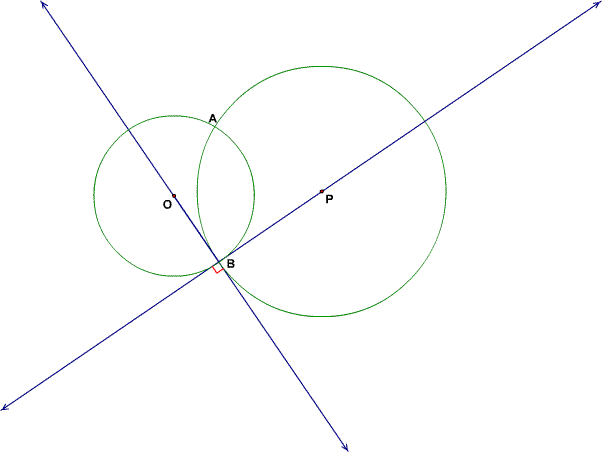
\includegraphics[scale=0.5]{orthocir}    
\end{center}

%------------------
%-- Message Achilleas ( moderator )
First, what shape do we expect to get?

%------------------
%-- Message Lucky0123 ( user )
% A circle

%------------------
%-- Message MathJams ( user )
% A circle

%------------------
%-- Message Wangminqi1 ( user )
% a circle

%------------------
%-- Message Riya_Tapas ( user )
% A circle

%------------------
%-- Message bryanguo ( user )
% a circle

%------------------
%-- Message Achilleas ( moderator )
We know the image of $O$ is a circle.

%------------------
%-- Message Achilleas ( moderator )
Do we know any points that this circle passes through?

%------------------
%-- Message coolbluealan ( user )
% A and B

%------------------
%-- Message MTHJJS ( user )
% A,B

%------------------
%-- Message Wangminqi1 ( user )
% $A$ and $B$

%------------------
%-- Message ca981 ( user )
% A and B

%------------------
%-- Message JacobGallager1 ( user )
% $A$ and $B$

%------------------
%-- Message dxs2016 ( user )
% A and B

%------------------
%-- Message bryanguo ( user )
% points A and B

%------------------
%-- Message mark888 ( user )
% $A$ and $B$

%------------------
%-- Message J4wbr34k3r ( user )
% A and B.

%------------------
%-- Message Riya_Tapas ( user )
% Points A and B

%------------------
%-- Message SlurpBurp ( user )
% $A$, $B$

%------------------
%-- Message Achilleas ( moderator )
We know it goes through A and B since A and B are on circle P.

%------------------
%-- Message Achilleas ( moderator )
Can you see which circle it is?

%------------------
%-- Message Achilleas ( moderator )
(Hint: We have not used orthogonality yet.)

%------------------
%-- Message MathJams ( user )
% circle O inverts to itself

%------------------
%-- Message JacobGallager1 ( user )
% So, the circle $O$ is preserved by inversion

%------------------
%-- Message MTHJJS ( user )
% circle O

%------------------
%-- Message AOPS81619 ( user )
% Is it the same as circle $O$?

%------------------
%-- Message Achilleas ( moderator )
We know that the image of circle O is perpendicular to P, so the radii of the image to points A and B are perpendicular to PA and PB.  Hence, the image of circle O is circle O.

%------------------
%-- Message Achilleas ( moderator )
Alternatively,  since the lines PA and PB are tangent to circle O, and they are fixed by the inversion, it follows that they will also be tangent to the image of circle O. Hence, the image of circle O is circle O.

%------------------
%-- Message Achilleas ( moderator )
Thus, a circle that is \textbf{orthogonal} to the circle we are inverting about is \textbf{fixed} under the inversion.

%------------------
%-- Message Achilleas ( moderator )
% Phewww...

%------------------
%-- Message Achilleas ( moderator )
\subsection{USING INVERSION ON OLYMPIAD PROBLEMS}

%------------------
%-- Message Riya_Tapas ( user )
% Problem time!

%------------------
%-- Message Achilleas ( moderator )
Now (finally) we are ready for some regular problems.

%------------------
%-- Message Achilleas ( moderator )
A couple general remarks on using inversion.  First, when you invert, you usually don't need to specify what circle you are inverting about, only its center.  Using a different circle will just result in a scaled diagram, which shouldn't make any difference.

%------------------
%-- Message Achilleas ( moderator )
Also, our last few facts give us some clues as to problems in which inversion might be useful.  Almost always, the problem must involve circles.  Usually, these circles will be tangent or orthogonal.  Also, there may be lines tangent to the circles.  And if you have a lot of lines and/or circles passing through the same point, that point is a good candidate for the center of inversion.

%------------------
%-- Message Achilleas ( moderator )
Inversion, as I noted at the beginning, seems a little magical, at least at first.  In general, you shouldn't ever spend a great deal of time trying it - usually it blows apart problems pretty quickly if it will work at all.  If you see a problem that feels like an inversion problem (probably because you've solved similar problems with inversion), try it briefly, but don't get too tied to it.

%------------------
%-- Message Achilleas ( moderator )
\begin{example}
Given a circle and two fixed points $A$ and $B$ on the circle, consider all possible of pairs of circles tangent to the given circle at $A$ and $B$ and to each other.  Find the locus of the point where the two new circles are tangent.    
\end{example}

%------------------
%-- Message Achilleas ( moderator )
% https://s3.amazonaws.com/classroom.artofproblemsolving.com/Classes/GeomOlympiad/Images/3tancirc.gif
\begin{center}
    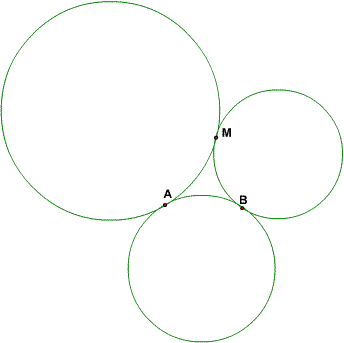
\includegraphics[scale=0.5]{3tancirc}    
\end{center}
%------------------
%-- Message Achilleas ( moderator )
What makes us think of inversion?

%------------------
%-- Message SlurpBurp ( user )
% tangent circles

%------------------
%-- Message smileapple ( user )
% circles and tangency

%------------------
%-- Message MathJams ( user )
% A ton of circles and tangencys

%------------------
%-- Message pritiks ( user )
% tangent circles

%------------------
%-- Message JacobGallager1 ( user )
% All the tangent circles

%------------------
%-- Message coolbluealan ( user )
% tangent circles

%------------------
%-- Message mark888 ( user )
% circles and tangents

%------------------
%-- Message Achilleas ( moderator )
We have circles galore, and they're all tangent.  We think of inversion because we know that we can invert tangent circles into parallel lines, which are easier to deal with than circles.

%------------------
%-- Message Achilleas ( moderator )
How can we invert tangent circles into parallel lines?

%------------------
%-- Message Achilleas ( moderator )
(we invert about a circle, not a point)

%------------------
%-- Message Riya_Tapas ( user )
% What are we inverting with respect to? Which circle

%------------------
%-- Message Achilleas ( moderator )
% This was my question. https://artofproblemsolving.com/assets/images/smilies/classroom-smile.gif

%------------------
%-- Message AOPS81619 ( user )
% A circle centered at the point of tangency

%------------------
%-- Message MathJams ( user )
% Invert about a circle with it's center as the tangency point

%------------------
%-- Message Achilleas ( moderator )
If we invert two tangent circles about a circle centered at the point of tangency, the image of the two circles will be two parallel lines (since the images are distinct lines and they can only intersect at the 'point at infinity'.

%------------------
%-- Message Achilleas ( moderator )
What should we choose as our center?  Should we choose point M (the point of tangency of the two new circles)?

%------------------
%-- Message MathJams ( user )
% We should choose A or B

%------------------
%-- Message coolbluealan ( user )
% A or B

%------------------
%-- Message Achilleas ( moderator )
Why not $M$?

%------------------
%-- Message JacobGallager1 ( user )
% We're trying to find the locus of $M$, so perhaps not? Our center of inversion should be a static point like A or B

%------------------
%-- Message coolbluealan ( user )
% we don't know where it is yet

%------------------
%-- Message MathJams ( user )
% Since we do not know where M is

%------------------
%-- Message smileapple ( user )
% $A$ and $B$ are fixed, whereas $M$ isn't

%------------------
%-- Message ca981 ( user )
% Not able to find locus of M

%------------------
%-- Message dxs2016 ( user )
% we're trying to find locus

%------------------
%-- Message Achilleas ( moderator )
We're not too happy with choosing M as the center of inversion, since that varies.  We're far more interested in seeing what happens to M under some other inversion, since then we might be able to say something about how M varies before inversion.

%------------------
%-- Message Achilleas ( moderator )
All that's left is inverting with respect to a circle centered at A or at B.  Let's choose A (doesn't matter which we choose).

%------------------
%-- Message Achilleas ( moderator )
If we invert about a circle centered at A with radius r, what will become of the two circles tangent at A?

%------------------
%-- Message Lucky0123 ( user )
% They become 2 parallel lines

%------------------
%-- Message JacobGallager1 ( user )
% They become parallel lines

%------------------
%-- Message ca981 ( user )
% Two parallel lines

%------------------
%-- Message Ezraft ( user )
% they will map to parallel lines

%------------------
%-- Message coolbluealan ( user )
% two parallel lines

%------------------
%-- Message MathJams ( user )
% two parallel lines

%------------------
%-- Message Achilleas ( moderator )
Circles passing through the center of inversion map to lines.  The images of circles tangent at the center of inversion are parallel lines, since the images can only intersect at the `point of infinity' (which is the image of their original intersection, the center of inversion).

%------------------
%-- Message Achilleas ( moderator )
Let's call these lines $m$ and $b$, with the image of $M$ (which we call $M'$ ) on $m$ and the image of $B (B' )$ on $b$.

%------------------
%-- Message Achilleas ( moderator )
That's pretty easy, all we have to worry about is the other circle.  What will its image be?

%------------------
%-- Message ca981 ( user )
% another circle

%------------------
%-- Message mustwin_az ( user )
% it will be a circle

%------------------
%-- Message coolbluealan ( user )
% a circle

%------------------
%-- Message MathJams ( user )
% Another circle

%------------------
%-- Message Achilleas ( moderator )
The image of a circle not passing through the center of inversion is another circle.

%------------------
%-- Message Achilleas ( moderator )
Do we know anything interesting about this image circle?

%------------------
%-- Message MTHJJS ( user )
% circle tangent to m, b

%------------------
%-- Message JacobGallager1 ( user )
% It will be a circle tangent to the two lines

%------------------
%-- Message Achilleas ( moderator )
The original circle through $B$ and $M$ was tangent to our original circles passing through $A$, so its image must be tangent to the images of those circles through $A$.  Hence, its image is tangent to both of our parallel lines $m$ and $b$.

%------------------
%-- Message Achilleas ( moderator )
How does this help?

%------------------
%-- Message JacobGallager1 ( user )
% This tells us that $M'B'$ is a diameter of the new circle

%------------------
%-- Message ca981 ( user )
% The circle is defined with diameter = distance between 2 parallel lines, and Passing M' and B'

%------------------
%-- Message Achilleas ( moderator )
We know that the image of $B$ is one of the tangency points of the image circle with the parallel lines.  Hence, if $B'$ is this image, we know our circle is tangent to $b$ at $B'$.  What does this tell us about $M'$?

%------------------
%-- Message Achilleas ( moderator )
$M'$ is the point on $m$ such that $B'M'$ is perpendicular to both $b$ and $m$:

%------------------
%-- Message Achilleas ( moderator )
% https://s3.amazonaws.com/classroom.artofproblemsolving.com/Classes/GeomOlympiad/Images/3taninv.gif
\begin{center}
    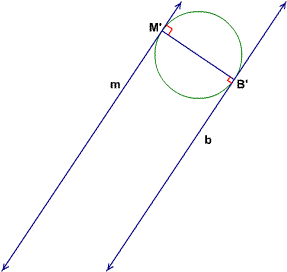
\includegraphics[scale=0.5]{3taninv}    
\end{center}

%------------------
%-- Message Achilleas ( moderator )
(Remember that $m$ and $M'$ here move while $b$ and $B'$ are fixed.)

%------------------
%-- Message Achilleas ( moderator )
How does this solve the problem?

%------------------
%-- Message Achilleas ( moderator )
Suppose for every possible pair of circles we perform this inversion with the same center and the same radius.  Line $b$ and point $B'$ are fixed - the inversion will always produce them exactly the same.  Point $M'$ will always appear on the other line such that $B'M'$ is perpendicular to line $b$.  Hence the locus of $M'$ is a line through $B'$ perpendicular to $b$.  Prove on your own why every point on this line is in the locus (other than $B'$ and the point at infinity).

%------------------
%-- Message Achilleas ( moderator )
Thus, what is the locus of $M$?

%------------------
%-- Message coolbluealan ( user )
% a circle

%------------------
%-- Message Achilleas ( moderator )
% How about a point on it?

%------------------
%-- Message Ezraft ( user )
% a circle that passes through $A$

%------------------
%-- Message ca981 ( user )
% B

%------------------
%-- Message coolbluealan ( user )
% B

%------------------
%-- Message MTHJJS ( user )
% A,B

%------------------
%-- Message Achilleas ( moderator )
We have found that the locus of the image of $M$ is a straight line not passing through the center of inversion.  Hence, the locus of $M$ is the inverse of the line's image.  The inverse of this line must be a circle through the center of inversion.

%------------------
%-- Message Achilleas ( moderator )
So that circle goes through $A$ and $B$.  Is there anything else we can say about it?

%------------------
%-- Message Achilleas ( moderator )
How is the new circle related to the original one?

%------------------
%-- Message coolbluealan ( user )
% orthogonal

%------------------
%-- Message ca981 ( user )
% orthogonal ?

%------------------
%-- Message MathJams ( user )
% orthogonal to our original circle

%------------------
%-- Message Achilleas ( moderator )
It is the circle through $A$ and $B$ that is orthogonal to the original circle.  We know this because the image of the locus of $M$ is orthogonal to $b$, so the locus of $M$ must be orthogonal to the inverse of $b$ (which is the original circle).

%------------------
%-- Message Achilleas ( moderator )
(Note that we have to exclude $A$ and $B$ themselves from the locus of $M$.)

%------------------
%-- Message Achilleas ( moderator )
Note also that the radius of inversion doesn't matter, so long as it's constant.

%------------------
%-- Message Achilleas ( moderator )
Last problem:

%------------------
%-- Message Achilleas ( moderator )
\begin{example}
Given two tangent circles and a point $P$ on their radical axis, construct with compass and ruler all the circles that are tangent to our original two circles and pass through the point $P$.
    
\end{example}

%------------------
%-- Message Achilleas ( moderator )
Why do we think of inversion?

%------------------
%-- Message Lucky0123 ( user )
% It has tangent circles

%------------------
%-- Message AOPS81619 ( user )
% tangency and circles

%------------------
%-- Message MathJams ( user )
% Tangency and circles and radical axis!

%------------------
%-- Message mark888 ( user )
% two tangent circles

%------------------
%-- Message Riya_Tapas ( user )
% Tangent circles

%------------------
%-- Message dxs2016 ( user )
% tangent circles

%------------------
%-- Message bryanguo ( user )
% because of the two tangent circles

%------------------
%-- Message Catherineyaya ( user )
% tangent and circles

%------------------
%-- Message Achilleas ( moderator )
We have tangent circles.  Also, point P is on the common tangent through the point of tangency of our two circles.

%------------------
%-- Message Achilleas ( moderator )
Thus we have 3 tangent figures, two circles and a line.  It's definitely worth thinking about inversion, even though it's a construction problem.

%------------------
%-- Message Achilleas ( moderator )
Here's what we're given:

%------------------
%-- Message Achilleas ( moderator )
% https://s3.amazonaws.com/classroom.artofproblemsolving.com/Classes/GeomOlympiad/Images/constinv.gif
\begin{center}
    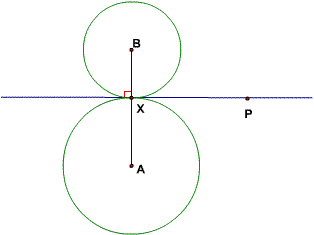
\includegraphics[scale=0.5]{constinv}    
\end{center}

%------------------
%-- Message Achilleas ( moderator )
We want the circles through P which are tangent to our other two circles.

%------------------
%-- Message Achilleas ( moderator )
It's not so obvious how to construct these circles.  Is it obvious how to construct any circles (or anything else, for that matter) which are tangent to both circles?

%------------------
%-- Message pritiks ( user )
% extend AB and draw a circle through the points it intersects with the circle

%------------------
%-- Message Achilleas ( moderator )
If we extend $AB$ to meet the circles again at $C$ and $D$, it's easy to construct the circle with diameter $CD$ - this one is tangent to both circles.

%------------------
%-- Message Achilleas ( moderator )
We also know how to construct the lines which are tangent to both circles.

%------------------
%-- Message Achilleas ( moderator )
Does either of these help us in our hunt for a circle through P which is tangent to the two circles?

%------------------
%-- Message Achilleas ( moderator )
Keeping in mind that we think inversion might be useful, can we find any way to relate any of our lines or circles we can construct to the circles we want?

%------------------
%-- Message Achilleas ( moderator )
What do we know about the images of two tangent objects under inversion?

%------------------
%-- Message Lucky0123 ( user )
% They are still tangent

%------------------
%-- Message JacobGallager1 ( user )
% They remain tangent

%------------------
%-- Message Achilleas ( moderator )
We know that the images of two tangent objects under inversion are themselves tangent.  How does this help?

%------------------
%-- Message Achilleas ( moderator )
We know that if we perform an inversion, it will map any circle or line that is tangent to both of our circles to something that is tangent to the images of our original circles.

%------------------
%-- Message Achilleas ( moderator )
So, do we just invert one of our tangent lines about P and voila - we have a circle tangent to our original circles?

%------------------
%-- Message MathJams ( user )
% No

%------------------
%-- Message Achilleas ( moderator )
Why not?

%------------------
%-- Message coolbluealan ( user )
% a circle tangent to the images of our original circles

%------------------
%-- Message Achilleas ( moderator )
The image of the tangent line will be tangent to the *images* of our circles.

%------------------
%-- Message Achilleas ( moderator )
But this does suggest another approach: what?

%------------------
%-- Message coolbluealan ( user )
% draw a tangent to the images of our original circle and then invert back

%------------------
%-- Message JacobGallager1 ( user )
% Take the image of the two circles under an inversion with center $P$. Draw common tangents from these images passing through the point $P$. Take the same inversion again, and you will have your desired circles

%------------------
%-- Message Achilleas ( moderator )
Invert both circles, find the two tangent lines to the *inverses*, and then invert back to get the circles we want.

%------------------
%-- Message Achilleas ( moderator )
That's a fine approach, and solves the problem.  To be a little more elegant though, we're actually going to choose a particular circle to invert around (centered at P) which leaves the original circles fixed and thus requires less work.

%------------------
%-- Message Achilleas ( moderator )
We need an inversion that leaves our circles unchanged.  What inversions leave circles unchanged?

%------------------
%-- Message Ezraft ( user )
% find an inversion such that circles $A$ and $B$ are the images

%------------------
%-- Message Achilleas ( moderator )
% How can we do that?

%------------------
%-- Message JacobGallager1 ( user )
% Orthogonal circles

%------------------
%-- Message MathJams ( user )
% Find a circle orthogonal to both circles

%------------------
%-- Message coolbluealan ( user )
% orthogonal circles

%------------------
%-- Message Achilleas ( moderator )
If two circles are orthogonal, then the image of each circle upon inverting about the other is itself.

%------------------
%-- Message JacobGallager1 ( user )
% Inverting about the circle centered at $P$ with radius $PX$ will leave the two circles fixed

%------------------
%-- Message Achilleas ( moderator )
Our inversion circle must be orthogonal to both circles since it must leave them unchanged.  Hence, we'll use a circle of inversion centered at $P$ with radius $PX$.

%------------------
%-- Message Achilleas ( moderator )
So, starting from just

%------------------
%-- Message Achilleas ( moderator )
% https://s3.amazonaws.com/classroom.artofproblemsolving.com/Classes/GeomOlympiad/Images/constinv.gif
\begin{center}
    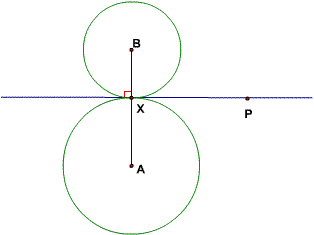
\includegraphics[scale=0.5]{constinv}    
\end{center}

%------------------
%-- Message Achilleas ( moderator )
How do we complete our construction?

%------------------
%-- Message coolbluealan ( user )
% construct a tangents to circle A and B, invert them with center P and radius PX

%------------------
%-- Message ca981 ( user )
% Draw common tangents of circle A and B

%------------------
%-- Message Achilleas ( moderator )
We construct our external tangents, and the circle with center P and radius XP:

%------------------
%-- Message Achilleas ( moderator )
% https://s3.amazonaws.com/classroom.artofproblemsolving.com/Classes/GeomOlympiad/Images/constinvstep.gif
\begin{center}
    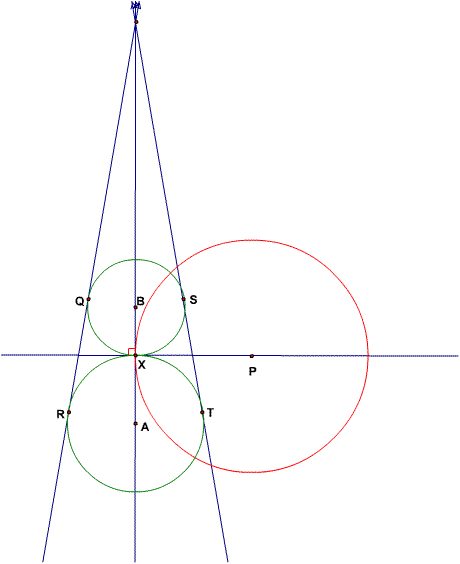
\includegraphics[scale=0.6]{constinvstep}    
\end{center}
%------------------
%-- Message Achilleas ( moderator )
How do we construct the inversions of the tangent lines?

%------------------
%-- Message MathJams ( user )
% Consider where points on these lines go

%------------------
%-- Message Achilleas ( moderator )
We know how to invert a point, so we can simply invert points to build our circle.  How many do we need to invert for each circle?

%------------------
%-- Message JacobGallager1 ( user )
% Just two, since we know they must also pass through $P$

%------------------
%-- Message MathJams ( user )
% 2 because it goes through P

%------------------
%-- Message Achilleas ( moderator )
We need only invert 2 points, as we know each image circle passes through P.  What points do we choose to invert and how can we construct their images quickly?

%------------------
%-- Message MathJams ( user )
% Invert the tangency points

%------------------
%-- Message mustwin_az ( user )
% invert S,T

%------------------
%-- Message Achilleas ( moderator )
We choose to invert Q and R to produce one circle, and S and T for the other.

%------------------
%-- Message Achilleas ( moderator )
How can we quickly find the image of R?

%------------------
%-- Message Achilleas ( moderator )
Do we know where it is on?

%------------------
%-- Message MathJams ( user )
% It is on circle A and  line PR

%------------------
%-- Message JacobGallager1 ( user )
% The second intersection of the line PR and the circle with center $A$

%------------------
%-- Message Achilleas ( moderator )
We know that the image of R must be on ray PR and that it must be on the lower circle (circle A), since the images of the inversions of QR and circle A must meet at the image of their intersection point (point R).

%------------------
%-- Message Achilleas ( moderator )
We can do the same to find the images of $Q, S,$ and $T$.  We call these images $R'$, $Q'$, $S'$, $T'$.  We then complete the problem by finding the circumcircles of $PR'Q'$ and $PS'T'$:

%------------------
%-- Message Achilleas ( moderator )
% https://s3.amazonaws.com/classroom.artofproblemsolving.com/Classes/GeomOlympiad/Images/constinv2cir.gif
\begin{center}
    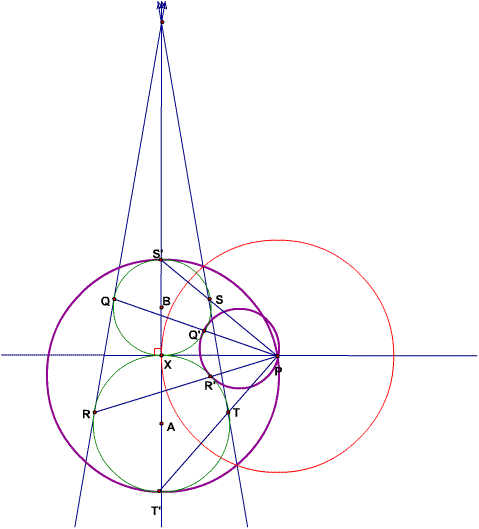
\includegraphics[scale=0.6]{constinv2cir}    
\end{center}

%------------------
%-- Message Achilleas ( moderator )
Both circles are shown in the figure.

%------------------
%-- Message Achilleas ( moderator )
Notice that we can use this approach to prove that there are at most 2 circles that fit the specifications of the problem (circle through P, tangent to the other two).

%------------------
%-- Message Achilleas ( moderator )
That's it for tonight.  With practice on the board and the final Challenge Set, you should get more used to using inversion in problems involving tangency.

%------------------
%-- Message Achilleas ( moderator )
Once again, don't spend forever with inversion on a problem. If it works, it usually works quickly.

%------------------
%-- Message Achilleas ( moderator )
If you don't get anywhere in 15 minutes, try something else (and I wouldn't reach for it first if something else, like homothety or good old angle chasing/power of a point looked good).

%------------------
%-- Message Achilleas ( moderator )
You could read about inversion in EGMO. I also like Stankova's exposition on inversion a lot!

%------------------
%-- Message Achilleas ( moderator )
See \url{https://mathcircle.berkeley.edu/sites/default/files/BMC6/ps0405/inversionSJ04.pdf}

%------------------
%-- Message Achilleas ( moderator )
There is another cool handout, by Dusan Dukic, one of the authors of the IMO compendium.

%------------------
%-- Message Achilleas ( moderator )
\url{https://memo.szolda.hu/feladatok/inversion_ddj.pdf}

%------------------
%-- Message Achilleas ( moderator )
You will see more Olympiad problems there!

%------------------
%-- Message MathJams ( user )
% what's after this class?

%------------------
%-- Message Achilleas ( moderator )
% Chaos.

%------------------
%-- Message pritiks ( user )
% lol

%------------------
%-- Message Ezraft ( user )
% https://artofproblemsolving.com/assets/images/smilies/classroom-boggle.gif

%------------------
%-- Message Achilleas ( moderator )
% https://artofproblemsolving.com/assets/images/smilies/classroom-smile.gif

%------------------
%-- Message Achilleas ( moderator )
There is no AoPS class after this one, other than WOOT.

%------------------
%-- Message Achilleas ( moderator )
There are many concepts/ideas/tools that we did not cover.

%------------------
%-- Message MathJams ( user )
% any recommended books?

%------------------
%-- Message Achilleas ( moderator )
One of my favorites is \emph{Solving Problems In Geometry: Insights And Strategies For Mathematical Olympiad And Competitions, by Kim Hoo Hang and Haibin Wang}.

What I like about it is that it gives insights about every solved example before presenting the neatly written solution to many math Olympiad problems. It includes ``a list of commonly used facts, useful skills, and problem-solving strategies and it will help you tackle challenging geometry problems at high-level Mathematics competitions."

You will learn a lot, but you won't find other useful stuff there, such as transformations, inversion, etc. But you will be well-equipped to move on to the students' favorite book in Olympiad geometry, which is EGMO by E.Chen.

%------------------
%-- Message Achilleas ( moderator )
Also, more importantly:

%------------------
%-- Message Achilleas ( moderator )
Solve problems...

%------------------
%-- Message Achilleas ( moderator )
Solve problems...

%------------------
%-- Message Achilleas ( moderator )
Solve problems...

%------------------
%-- Message Achilleas ( moderator )
And...study new stuff.

%------------------
%-- Message Achilleas ( moderator )
% I guess that's really it for today!

%------------------
%-- Message Achilleas ( moderator )
% Do not forget our survey. Thank you all! See you around! It was great teaching this class! 

%------------------
